% \documentclass[table]{beamer}
\documentclass[table,handout]{beamer}
\setbeameroption{show notes}
% \setbeameroption{hide notes}
% \setbeameroption{show only notes}
\usepackage{varwidth}

\newif\ifhide
\newif\ifpost
\newif\ifhideclicker

% \hidetrue
% \hideclickertrue
% \posttrue

\newcommand{\whiteout}[1]{\textcolor{white}{#1}}
% \newcommand{\whiteoutbox}[1]{\fcolorbox{white}{white}{\parbox{\dimexpr \linewidth-2\fboxsep-2\fboxrule}{\whiteout{#1}}}}
% \newcommand{\notebox}[1]{\fcolorbox{blue}{white}{\parbox{\dimexpr \linewidth-2\fboxsep-2\fboxrule}{#1}}}
\newcommand{\whiteoutbox}[1]{\fcolorbox{white}{white}{\parbox{\linewidth}{\whiteout{#1}}}}
\newcommand{\notebox}[1]{\fcolorbox{blue}{white}{\parbox{\linewidth}{#1}}}
\newcommand{\blankbox}[1]{\phantom{\varwidth{\linewidth}\whiteoutbox{#1}\endvarwidth}}
\newcommand{\blank}[1]{\phantom{\varwidth{\linewidth}#1\endvarwidth}}

\ifhide%
    \newcommand{\hmask}[1]{\blank{#1}}%
\else%
    \newcommand{\hmask}[1]{#1}%
\fi

\ifhide%
    \newcommand{\wout}[1]{\whiteout{#1}}%
\else%
    \newcommand{\wout}[1]{#1}%
\fi

\ifhide%
    \newcommand{\hignore}[1]{}%
\else%
    \newcommand{\hignore}[1]{#1}%
\fi

\ifpost%
    \newcommand{\nopost}[1]{}%
\else%
    \newcommand{\nopost}[1]{#1}%
\fi

\ifhideclicker%
    \newcommand{\clickerslide}[1]{\stepcounter{clickerQuestionCounter}%
        \begin{frame}[t]
            \textcolor{blue}{Q \arabic{clickerQuestionCounter}:}
        \end{frame}}
\else%
    \newcommand{\clickerslide}[1]{#1}%
\fi

\ifhide%
    \newcommand{\hidebox}[1]{\blank{#1}}%
\else%
    \newcommand{\hidebox}[1]{\notebox{#1}}%
\fi

\ifhide%
    \newcommand{\wbox}[1]{\whiteoutbox{#1}}%
\else%
    \newcommand{\wbox}[1]{\notebox{#1}}%
\fi

\ifhide%
    \newcommand{\nbox}[1]{\blankbox{#1}}%
\else%
    \newcommand{\nbox}[1]{\notebox{#1}}%
\fi

\ifhideclicker%
    \newcommand{\clickeranswer}[1]{#1}%
\else%
    \ifhide%
        \newcommand{\clickeranswer}[1]{#1}%
    \else%
        \newcommand{\clickeranswer}[1]{\textbf{\textcolor{blue}{#1}}}%
    \fi
\fi

\usepackage{beamerthemesplit}
% \usetheme{boxes}
\usetheme{Malmoe}
\usecolortheme{seahorse}
% \usecolortheme{seagull}
\usepackage{ifthen}
\usepackage{xspace}
\usepackage{multirow}
\usepackage{multicol}
\usepackage{booktabs}
\usepackage{xcolor}
\usepackage{wasysym}
\usepackage{comment}
\usepackage{hyperref}
\hypersetup{pdfborder={0 0 0}, colorlinks=true, urlcolor=blue, linkcolor=blue, citecolor=blue}
\usepackage{changepage}
\usepackage[compatibility=false]{caption}
\captionsetup[figure]{font=scriptsize, labelformat=empty, textformat=simple, justification=centering, skip=2pt}
\usepackage{tikz}
\usetikzlibrary{trees,calc,backgrounds}

\usepackage[bibstyle=joaks-slides,maxcitenames=3,mincitenames=1,backend=biber]{biblatex}

\newrobustcmd*{\shortfullcite}{\AtNextCite{\renewbibmacro{title}{}\renewbibmacro{in:}{}\renewbibmacro{number}{}}\fullcite}

\newrobustcmd*{\footlessfullcite}{\AtNextCite{\renewbibmacro{title}{}\renewbibmacro{in:}{}}\footfullcite}

% Make all footnotes smaller
% \renewcommand{\footnotesize}{\scriptsize}

\definecolor{myGray}{gray}{0.9}
\colorlet{rowred}{red!30!white}

\setbeamertemplate{blocks}[rounded][shadow=true]

\setbeamercolor{defaultcolor}{bg=structure!30!normal text.bg,fg=black}
\setbeamercolor{block body}{bg=structure!30!normal text.bg,fg=black}
\setbeamercolor{block title}{bg=structure!50!normal text.bg,fg=black}

\newenvironment<>{varblock}[2][\textwidth]{%
  \setlength{\textwidth}{#1}
  \begin{actionenv}#3%
    \def\insertblocktitle{#2}%
    \par%
    \usebeamertemplate{block begin}}
  {\par%
    \usebeamertemplate{block end}%
  \end{actionenv}}

\newenvironment{displaybox}[1][\textwidth]
{
    \centerline\bgroup\hfill
    \begin{beamerboxesrounded}[lower=defaultcolor,shadow=true,width=#1]{}
}
{
    \end{beamerboxesrounded}\hfill\egroup
}

\newenvironment{onlinebox}[1][4cm]
{
    \newbox\mybox
    \newdimen\myboxht
    \setbox\mybox\hbox\bgroup%
        \begin{beamerboxesrounded}[lower=defaultcolor,shadow=true,width=#1]{}
    \centering
}
{
    \end{beamerboxesrounded}\egroup
    \myboxht\ht\mybox
    \raisebox{-0.25\myboxht}{\usebox\mybox}\hspace{2pt}
}

\newenvironment{mydescription}{
    \begin{description}
        \setlength{\leftskip}{-1.5cm}}
    {\end{description}}

\newenvironment{myitemize}{
    \begin{itemize}
        \setlength{\leftskip}{-.3cm}}
    {\end{itemize}}

% footnote without a marker
\newcommand\barefootnote[1]{%
  \begingroup
  \renewcommand\thefootnote{}\footnote{#1}%
  \addtocounter{footnote}{-1}%
  \endgroup
}

% define formatting for footer
\newcommand{\myfootline}{%
    {\it
    \insertshorttitle
    \hspace*{\fill} 
    \insertshortauthor, \insertshortinstitute
    % \ifx\insertsubtitle\@empty\else, \insertshortsubtitle\fi
    \hspace*{\fill}
    \insertframenumber/\inserttotalframenumber}}

% set up footer
\setbeamertemplate{footline}{%
    \usebeamerfont{structure}
    \begin{beamercolorbox}[wd=\paperwidth,ht=2.25ex,dp=1ex]{frametitle}%
        % \Tiny\hspace*{4mm}\myfootline\hspace{4mm}
        \tiny\hspace*{4mm}\myfootline\hspace{4mm}
    \end{beamercolorbox}}

% remove navigation bar
\beamertemplatenavigationsymbolsempty

\makeatletter
    \newenvironment{noheadline}{
        \setbeamertemplate{headline}[default]
        \def\beamer@entrycode{\vspace*{-\headheight}}
    }{}
\makeatother

\newcounter{clickerQuestionCounter}
\ifhideclicker%
\newenvironment{clickerquestion}
{ \stepcounter{clickerQuestionCounter}
  \begin{enumerate}[Q \arabic{clickerQuestionCounter}:]\color{white} }
{ \end{enumerate} }
\else%
\newenvironment{clickerquestion}
{ \stepcounter{clickerQuestionCounter}
  \begin{enumerate}[Q \arabic{clickerQuestionCounter}:] }
{ \end{enumerate} }
\fi

\ifhideclicker%
\newenvironment{clickeroptions}
{ \begin{enumerate}[\begingroup\color{white} 1)\endgroup]\color{white} }
{ \end{enumerate} }
\else%
\newenvironment{clickeroptions}
{ \begin{enumerate}[\begingroup\color{red} 1)\endgroup] }
{ \end{enumerate} }
\fi


\tikzstyle{centered} = [align=center, text centered, font=\sffamily\bfseries]
\tikzstyle{skip} = [centered, inner sep=0pt, fill]
\tikzstyle{empty} = [centered, inner sep=0pt]
\tikzstyle{inode} = [centered, circle, minimum width=4pt, fill=black, inner sep=0pt]
\tikzstyle{tnode} = [centered, circle, inner sep=1pt]
\tikzset{
  % edge styles
  level distance=10mm,
  mate/.style={edge from parent/.style={draw,distance=3pt}},
  mleft/.style={grow=left, level distance=10mm, edge from parent path={(\tikzparentnode.west)--(\tikzchildnode.east)}},
  mright/.style={grow=right, level distance=10mm, edge from parent path={(\tikzparentnode.east)--(\tikzchildnode.west)}},
  % node styles
  male/.style={rectangle,minimum size=4mm,fill=gray!80},
  female/.style={circle,minimum size=4mm,fill=gray!80},
  amale/.style={male,fill=red},
  afemale/.style={female,fill=red},
}

\newcommand{\highlight}[1]{\textcolor{violet}{\textit{\textbf{#1}}}}
\newcommand{\super}[1]{\ensuremath{^{\textrm{\sffamily #1}}}}
\newcommand{\sub}[1]{\ensuremath{_{\textrm{\sffamily #1}}}}
\newcommand{\dC}{\ensuremath{^\circ{\textrm{C}}}}
\newcommand{\tb}{\hspace{2em}}
\providecommand{\e}[1]{\ensuremath{\times 10^{#1}}}
\newcommand{\myHangIndent}{\hangindent=5mm}

\newcommand{\spp}[1]{\textit{#1}}

\newcommand\mybullet{\leavevmode%
\usebeamertemplate{itemize item}\hspace{.5em}}

\makeatletter
\newcommand*{\rom}[1]{\expandafter\@slowromancap\romannumeral #1@}
\makeatother

\newcommand{\blankslide}{{\setbeamercolor{background canvas}{bg=black}
\setbeamercolor{whitetext}{fg=white}
\begin{frame}<handout:0>[plain]
\end{frame}}}

\newcommand{\whiteslide}{
\begin{frame}<handout:0>[plain]
\end{frame}}

\newcommand{\f}[1]{\ensuremath{F_{#1}}}
\newcommand{\x}[1]{X\ensuremath{^{#1}}}
\newcommand{\y}[1]{Y\ensuremath{^{#1}}}

% Population growth macros
\newcommand{\popsize}[1]{\ensuremath{N_{#1}}}
\newcommand{\popgrowthratediscrete}[1]{\ensuremath{\lambda_{#1}}}
\newcommand{\popgrowthrate}[1]{\ensuremath{r_{#1}}}
\newcommand{\ptime}{\ensuremath{t}\xspace}

\tikzset{hide on/.code={\only<#1>{\color{white}}}}
\tikzset{
    invisible/.style={opacity=0},
    visible on/.style={alt={#1{}{invisible}}},
    alt/.code args={<#1>#2#3}{%
        \alt<#1>{\pgfkeysalso{#2}}{\pgfkeysalso{#3}}
        % \pgfkeysalso doesn't change the path
    },
}

% \bibliography{../bib/references}
\bibliography{references}
\author[J.\ Oaks]{
    %Jamie R.\ Oaks\inst{1}
    Jamie R.\ Oaks
}
\institute[BIOL 180]{
    \inst{}%
        BIOL 180: Introductory Biology
}



\title[Population Structure]{Population Structure}
% \date{\today}
\date{May 18, 2015}

\begin{document}

\begin{noheadline}
\maketitle
\end{noheadline}

\nopost{
\begin{noheadline}
\begin{frame}[c]
    \vspace{-6mm}
    \begin{center} 
        \includegraphics[height=1.2\textheight]{../images/seating-chart-2.pdf}
    \end{center}
\end{frame}
\end{noheadline}
}


\clickerslide{
\begin{noheadline}
\begin{frame}
    \begin{clickerquestion}
        \item When the AIDS epidemic was at its height, the U.N.'s population
            division had to revise its population projections downward.
            Compared to other diseases, why would AIDS have an especially large
            effect on population size?  

        \begin{clickeroptions}
            \item It is an infectious disease.
            \item \clickeranswer{It is fatal, and afflicts people of
                    reproductive age.}
            \item It is a sexually transmitted disease. 
            \item Most diseases kill the very old and very young. 
            \item At the time, there was no effective treatment. 
        \end{clickeroptions}
    \end{clickerquestion}
    \nbox{Key concept = not only removing infected individuals, but their
        offspring}
\end{frame}
\end{noheadline}
}

\begin{noheadline}
\begin{frame}
\frametitle{Today's issues:}
\vspace{5mm}
% \tableofcontents[subsectionstyle=hide]
\tableofcontents
\end{frame}
\end{noheadline}

\section{How does age structure affect population dynamics?}

\begin{frame}[t]
    \begin{adjustwidth}{-2em}{-1.5em}

    \vspace{-3mm}

    \begin{columns}[t]
    
    \column{0.5\linewidth}

    \textbf{I. How does age structure affect population dynamics?} \\

    \vspace{0.3cm}
    Using population pyramids to characterize age structure and assess
    prospects for population growth.\\

    \uncover<2->{
    \vspace{0.3cm}
    Why assess the following?  
    }

    \column{0.5\linewidth}

    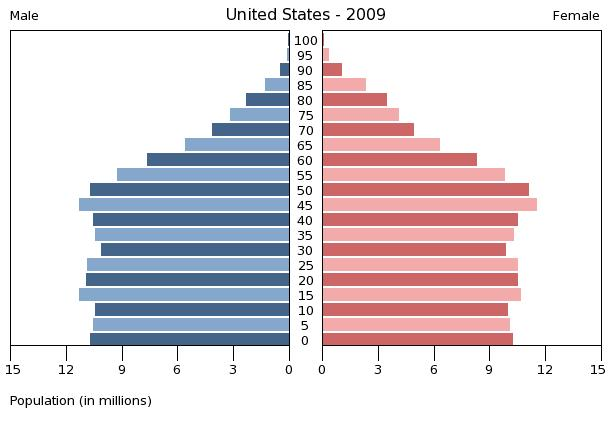
\includegraphics[width=1\columnwidth]{../images/pop-pyramid-usa-2009.png}

    \end{columns}

    \uncover<2->{
    \begin{itemize}
        \item Relative number of newly born/hatched/germinated \\

            \nbox{Use for predicting growth when the offspring reach
                reproductive age}
    
        \vspace{2mm}
        \item Relative number near or at peak reproductive age \\

            \nbox{Use for predicting current growth}
    
        \vspace{2mm}
        \item Relative number of old/post-reproductive \\

            \nbox{Use to determine what proportion of the population cannot
                contribute to growth}
    \end{itemize}
    }

    \end{adjustwidth}
\end{frame}

\begin{frame}[t]
    \frametitle{Age pyramids}
    \begin{adjustwidth}{-2em}{-1.5em}
        \begin{itemize}
            \item There are three basic patterns
        \end{itemize}

    \begin{columns}
        \column{0.33\linewidth}
            \begin{figure}
                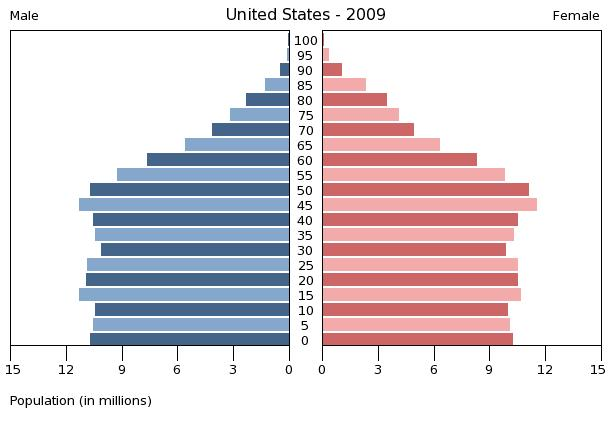
\includegraphics[width=1\columnwidth]{../images/pop-pyramid-usa-2009.png}
                \caption{\large USA}
            \end{figure}
        \column{0.33\linewidth}
            \begin{figure}
                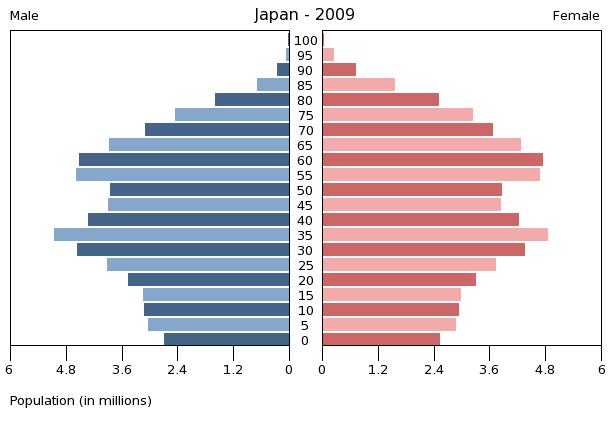
\includegraphics[width=1\columnwidth]{../images/pop-pyramid-japan-2009.png}
                \caption{\large Japan}
            \end{figure}
        \column{0.33\linewidth}
            \begin{figure}
                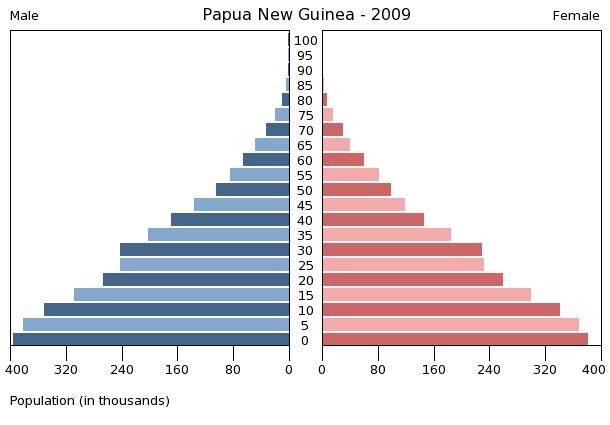
\includegraphics[width=1\columnwidth]{../images/pop-pyramid-png-2009.png}
                \caption{\large PNG}
            \end{figure}
    \end{columns}
    \end{adjustwidth}
\end{frame}

\clickerslide{
\begin{frame}
    \begin{adjustwidth}{-2em}{-1.5em}
    \begin{columns}
        \column{0.33\linewidth}
            \begin{figure}
                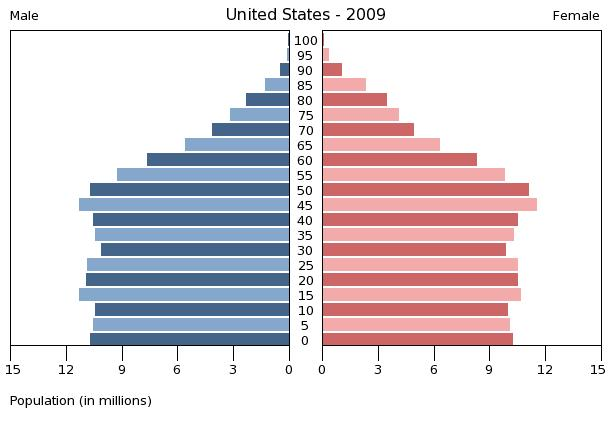
\includegraphics[width=1\columnwidth]{../images/pop-pyramid-usa-2009.png}
                \caption{\large USA}
            \end{figure}
        \column{0.33\linewidth}
            \begin{figure}
                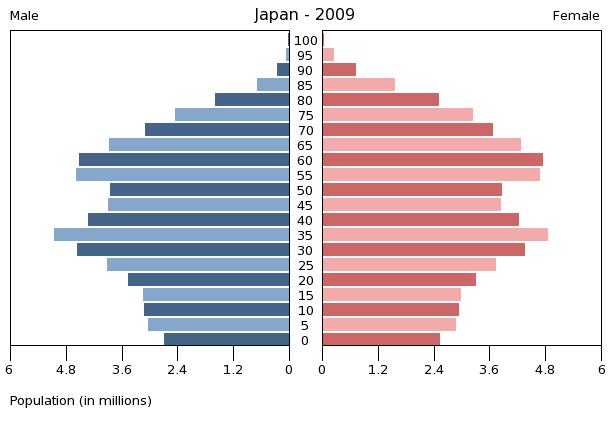
\includegraphics[width=1\columnwidth]{../images/pop-pyramid-japan-2009.png}
                \caption{\large Japan}
            \end{figure}
        \column{0.33\linewidth}
            \begin{figure}
                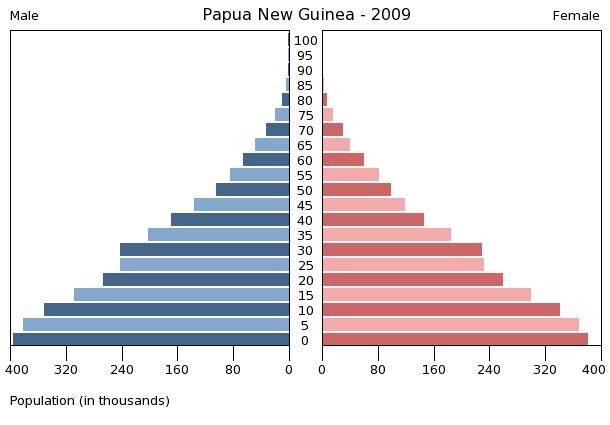
\includegraphics[width=1\columnwidth]{../images/pop-pyramid-png-2009.png}
                \caption{\large PNG}
            \end{figure}
    \end{columns}

    \end{adjustwidth}

    \begin{clickerquestion}
        \item Which of the following best describes the growth of these
            populations as of 2009?
    \end{clickerquestion}
    \begin{table}%[htbp]
        % \addtolength{\tabcolsep}{-0.09cm}
        \centering
        \begin{tabular}{ l l l l }
            \toprule
             & USA & Japan & PNG \\
            \hline
            \textcolor{red}{1)} & \clickeranswer{$\approx 0$ growth} & \clickeranswer{Declining population} & \clickeranswer{Rapid growth} \\ 
            \textcolor{red}{2)} & Slow growth & Slow growth & $\approx 0$ growth \\ 
            \textcolor{red}{3)} & Slow grouth & Declining population & Slow growth \\ 
            \textcolor{red}{4)} & $\approx 0$ growth & $\approx 0$ growth & Rapid growth \\ 
            \bottomrule
        \end{tabular}
    \end{table}
\end{frame}
}

\begin{frame}[t]
    \begin{adjustwidth}{-2em}{-1.5em}

    \textbf{What do you notice about these graphs?} \\

    % \vspace{-8mm}
    % \begin{columns}
    %     \column{0.5\textwidth}
    %         \begin{figure}
    %             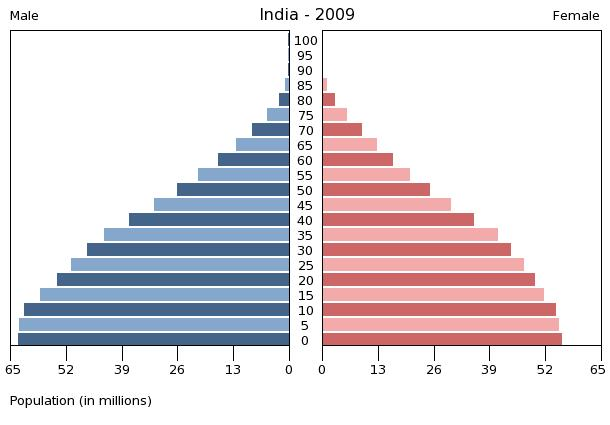
\includegraphics[width=1.1\columnwidth]{../images/pop-pyramid-india-2009.png}
    %             \caption{\large India 2009}
    %         \end{figure}
    %     \column{0.5\textwidth}
    %         \begin{figure}
    %             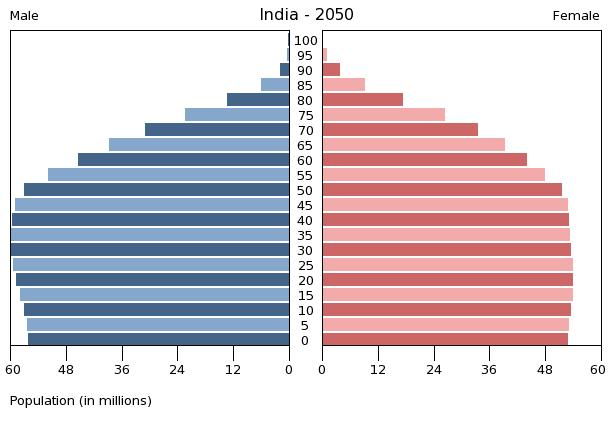
\includegraphics[width=1.1\columnwidth]{../images/pop-pyramid-india-2050.png}
    %             \caption{\large India 2050}
    %         \end{figure}
    % \end{columns}
    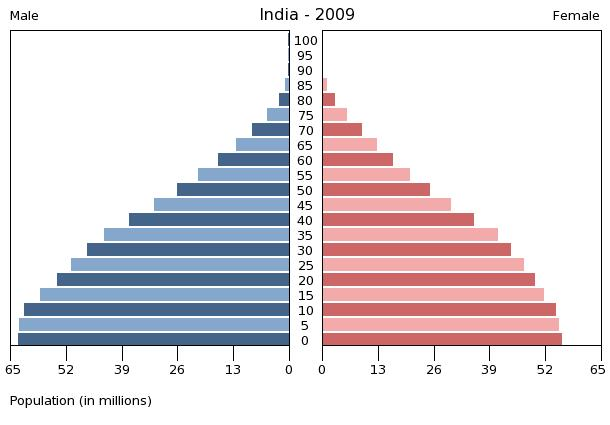
\includegraphics[width=0.51\linewidth]{../images/pop-pyramid-india-2009.png}
    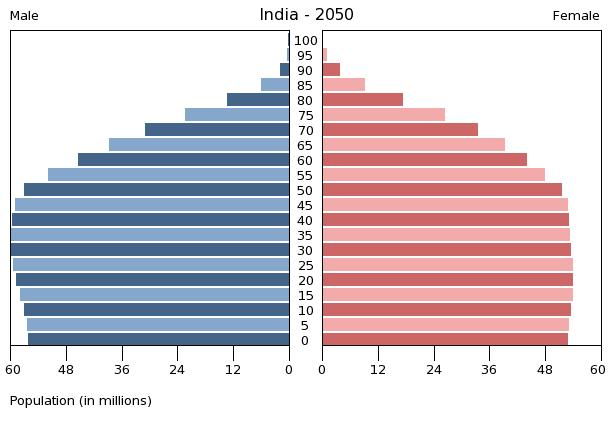
\includegraphics[width=0.51\linewidth]{../images/pop-pyramid-india-2050.png}

    \nbox{There are many more men than women (e.g., for ages 1--24 on left,
        there are 32,700,000 more men than women!).}

    \nbox{There is a shift from rapid growth (current; left) to a stable or
        slightly declining population (future; right).}
    \end{adjustwidth}
\end{frame}

\clickerslide{
\begin{frame}[t]
    \begin{adjustwidth}{-2em}{-1.5em}

    \vspace{-6mm}
    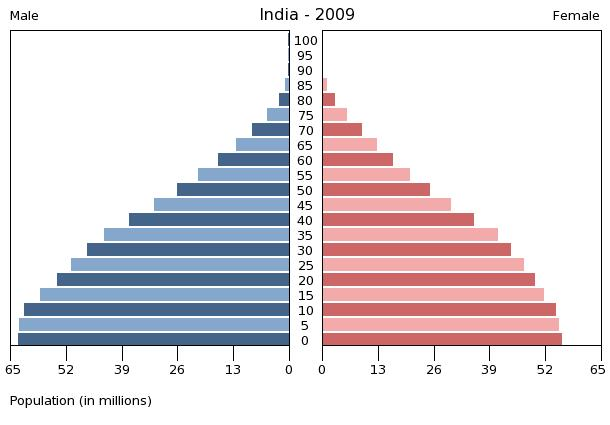
\includegraphics[width=0.51\linewidth]{../images/pop-pyramid-india-2009.png}
    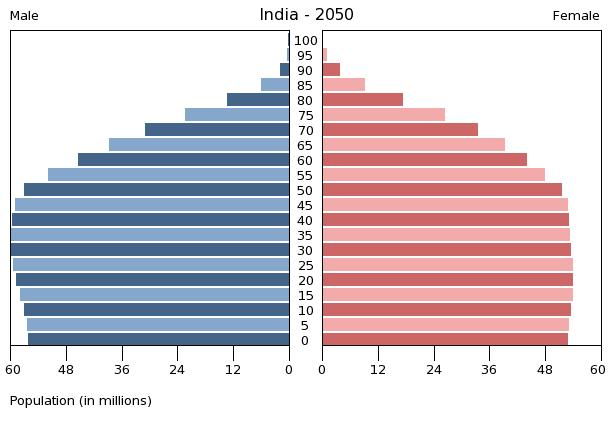
\includegraphics[width=0.51\linewidth]{../images/pop-pyramid-india-2050.png}

    \vspace{-2mm}
    \begin{clickerquestion}
        \item Which of the following statements is NOT supported by these data?
 
        \begin{clickeroptions}
            \item In 2050, most senior citizens (age 65+) will be female.
            \item India's population has been booming for the past 50 years.
            \item Since about 1985, there has been a very strongly male-biased
                sex ratio at birth.
            \item \clickeranswer{The incentive-based sterilization program,
                    which took place in 1976, had a dramatic impact on
                    fertility and growth rates.}
            \item Fertility rates are starting to drop; by 2050, population
                growth will be low or 0.
        \end{clickeroptions}
    \end{clickerquestion}
    \end{adjustwidth}
    \note[item]{Program used propaganda and monetary incentives. In 2002--2003,
        114k vasectomies and 4.6 million tubal ligations.}
\end{frame}
}


\section{How does geographic structure affect population dynamics?}

% \begin{noheadline}
% \begin{frame}
% \frametitle{Today's issues:}
% \tableofcontents[subsectionstyle=hide,currentsection]
% \end{frame}
% \end{noheadline}

\begin{frame}[t]
    % \frametitle{Geographic ranges of species}

    \begin{adjustwidth}{-2em}{-1.5em}

    \vspace{-3mm}
    II. How does geographic structure affect population dynamics? \\

    % \vspace{0.5cm}
    % Range maps \ldots \\

    \vspace{-3mm}
    \begin{columns}
        \column{0.5\textwidth}

        \column{0.5\textwidth}

        \begin{figure}
            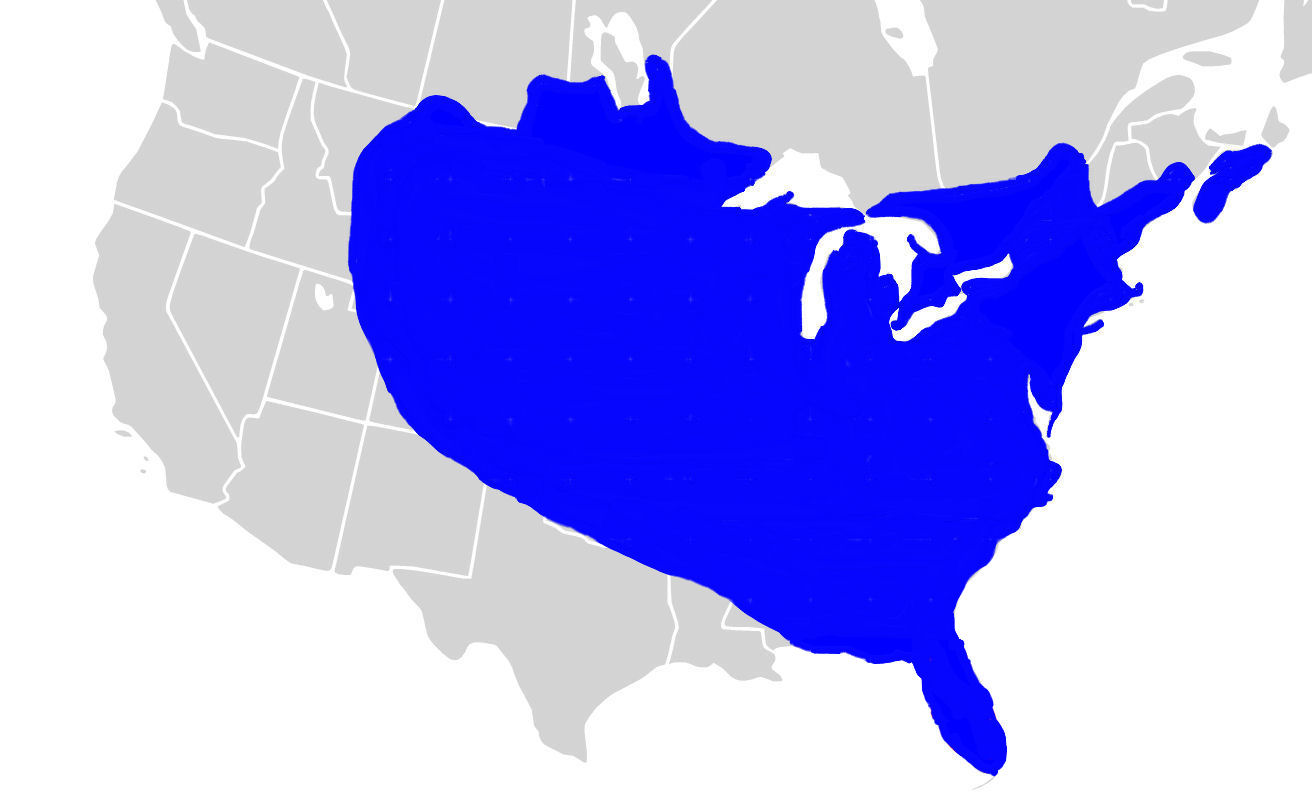
\includegraphics[width=1.1\textwidth]{../images/snapping-turtle-range-cc-by-sa-30-DGE-Robertson.png}
            \caption{Common snapping turtle range map.
                {\tiny
                \href{http://creativecommons.org/licenses/by-sa/3.0/}{CC BY-SA 3.0}
                \href{http://upload.wikimedia.org/wikipedia/commons/f/f9/Common_snapping_turtle_range_map.jpg}{D.G.E Robertson}.}
            }
        \end{figure}

    \end{columns}

    \uncover<2->{
    What factors might determine the range of snapping turtles? \\
    \nbox{Abiotic factors: plate tectonics, temperature, rainfall, geography,
        watersheds, substrate, water flow, etc.}
    \nbox{Biotic factors: Availability of food, presence of competitors,
        predators, parasites, etc.}
    }

    \end{adjustwidth}
\end{frame}

\begin{frame}[t]
    \begin{adjustwidth}{-2em}{-1.5em}
    Geographic patterns of species ranges \ldots \\

    \vspace{0.5cm}
    What factors would lead to the following distribution patterns? \\

    \begin{itemize}
        \item Clumped: \\
            \nbox{Quality of habitat is patchy; Social behavior; Absence of
                inter-specific competitors or predators is patchy.}

        \item Overdispersed (``uniform''): \\
            \nbox{Negative intra-specific interactions. E.g., competition among
                individuals for space or resources.}

        \item Random: \\
            \nbox{Quality of habitat is roughly even, and individuals occur
                independently of one another.}
    \end{itemize}

    \uncover<2->{
    Are these patterns mutually exclusive? (Hint: think across spatial scales)

    \nbox{No. E.g., the same species can have be overdispersed locally (on
        small spatial scale), but distributed in a clumpy pattern regionally
        (at larger spatial scales).}
    }
    \end{adjustwidth}
    \note[item]{Use volunteers to demonstrate the three patterns; All stand as
        close to a few sheets of paper as possible (clumpy); Stay as far apart
        as possible (overdispersed); What is the NULL? (random.}
\end{frame}

\clickerslide{
\begin{frame}
    \begin{clickerquestion}
        \item Which of the following best characterizes species ranges?
        \begin{clickeroptions}
            \item Ranges are static, because despite the flux in biotic factors,
                abiotic factors are mostly constant over time.
            \item \clickeranswer{Ranges are dynamic, because abiotic and biotic
                    factors change over time.}
            \item Ranges are static, because despite the flux in abiotic factors,
                biotic factors are mostly constant over time.
            \item Individuals tend to be overdispersed in order to best
                share resources across the species.
        \end{clickeroptions}
    \end{clickerquestion}
\end{frame}
}

\begin{frame}[t]
    \begin{adjustwidth}{-2em}{-1.5em}
    \begin{description}
        \item[Metapopulation:] \ \\
            \nbox{A population of populations connected by migration.}
    \end{description}

    \uncover<2->{
    \vspace{3mm}
    \begin{columns}[t]

        \column{0.35\textwidth}

        E.g., Glanville fritillaries on the \r{A}land Islands in the Baltic
        Sea.
        \href{http://www.helsinki.fi/science/metapop/Field_sites/Aland.html}{Hanski
            et al.}

        \vspace{5mm}
        Caterpillars require meadows with certain host plants

        \column{0.64\textwidth}

        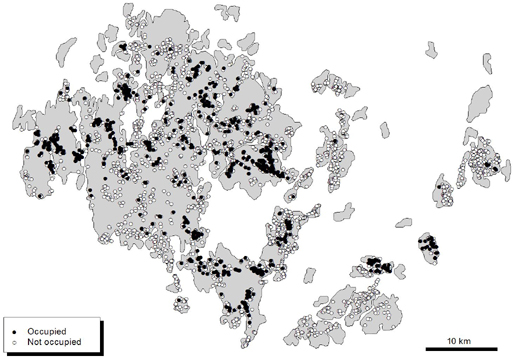
\includegraphics[width=1.0\columnwidth]{../images/fritillaries-metapopulation.png}

    \end{columns}
    }
    \end{adjustwidth}
\end{frame}

\begin{frame}[t]
    % \frametitle{Exploring metapopulation dynamics---
    %     \href{http://www.helsinki.fi/science/metapop/Field_sites/Aland.html}{Hanski
    %         et al.}}
    \begin{adjustwidth}{-2em}{-1.5em}

    \vspace{-3mm}
    How do metapopulations work?
    \href{http://www.helsinki.fi/science/metapop/Field_sites/Aland.html}{Hanski
        et al.}

    \vspace{-2mm}
    \begin{columns}

    \column{0.52\textwidth}

    \begin{itemize}
            \small
        \item<1-> Conduct census, marking 1731 individuals
        \item<2-> Later in season, re-capture 741
            \begin{itemize}
                \item 9\% were found in previously unoccupied patch
            \end{itemize}
        \item<3-> Conduct census 2 years later
            \begin{itemize}
                \item Some populations extinct, and other patches newly
                    colonized
            \end{itemize}
    \end{itemize}

    \column{0.5\textwidth}

    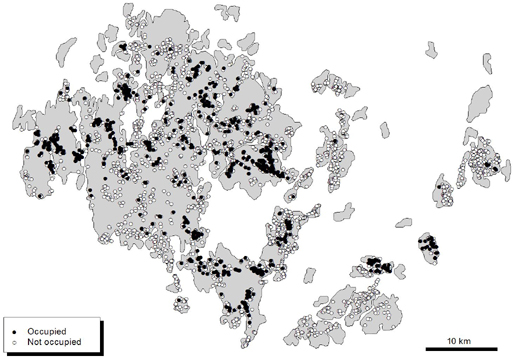
\includegraphics[width=1.0\columnwidth]{../images/fritillaries-metapopulation.png}

    \end{columns}

    \vspace{3mm}
    \uncover<4->{Punchlines: \\
    \nbox{\scriptsize Migration (gene flow) from patch to patch. Local
        populations are frequently going extinct, and empty patches are being
        colonized. Migration among patches is critical to maintain the
        metapopulation as a whole. I.e., for the metapopulation as a whole, the
        suitable patches of habitat that are currently NOT supporting the
        caterpillars are just as important as the patches that currently
        contain the caterpillars}}

    \end{adjustwidth}
\end{frame}

\clickerslide{
\begin{frame}
    \begin{clickerquestion}
        \item In the early 2000s, federal officials removed protective
            regulations on streams in the Pacific Northwest that did not
            contain salmon, even though the habitat was appropriate. As a
            biologist, comment. 
 
        \begin{clickeroptions}
            \item Populations in a metapopulation go extinct naturally, so it's
                ok to let some habitats be developed. 
            \item These streams are important ``habitat corridors'' that allow
                gene flow between isolated populations.
            \item \clickeranswer{This is a bad idea---it's important to save
                    habitat that might be colonized later.}
            \item This is a good move; federal resources should be focused on
                captive breeding, as metapopulations are doomed. 
        \end{clickeroptions}
    \end{clickerquestion}
\end{frame}
}

\begin{frame}[t]
    \begin{adjustwidth}{-2em}{-1.5em}

    \vspace{-3mm}
    Humans are fragmenting habitats and forcing many populations into a
    metapopulation structure with limited migration. How will this affect: \\

    \begin{itemize}
        \item Inbreeding:

            \nbox{Will increase---small populations with low gene flow}

            \vspace{8mm}
        \item Genetic drift:

            \nbox{Will increase---small populations with low gene flow will
                lead to more random changes in allele frequencies}

            \vspace{2mm}
        \item Genetic diversity:

            \nbox{Will decrease---losing alleles via drift}

            \vspace{8mm}
        \item Range changes in response to climate change:

            \nbox{Many species will have a more difficult time tracking
                favorable environmental conditions---cannot disperse through
                developed areas}
    \end{itemize}
    \end{adjustwidth}
\end{frame}

% \section{What regulates populations?}


\end{document}

\clickerslide{
\begin{frame}
    \begin{clickerquestion}
        \item 
        \begin{clickeroptions}
            \item 
            \item 
            \item 
            \item 
        \end{clickeroptions}
    \end{clickerquestion}
\end{frame}
}

\clickerpost{
{
\usebackgroundtemplate{\includegraphics[page=17,width=\paperwidth]{./24-Radiation-extinction.pdf}}
\begin{frame}[t,plain]
    \begin{adjustwidth}{-2em}{-1.5em}
        \cmask{Answer: 3}
    \end{adjustwidth}
\end{frame}
}
}

